\documentclass[a4paper]{article}
\usepackage[utf8]{inputenc}
\usepackage[english]{babel}
\usepackage{amsmath} % per ambienti tipo cases
\usepackage{amssymb}
\usepackage{mathtools}
\usepackage{siunitx}
\usepackage{graphicx} % per includere figure
%\usepackage{subfigure}
\usepackage{wrapfig}
\usepackage{booktabs} % per le tabelle
\usepackage{caption}
\usepackage{fancyhdr}
\usepackage{hyperref}
\usepackage[section]{placeins}
\usepackage{microtype}
\usepackage{caption}
\usepackage{subcaption}
\usepackage{listings}
\usepackage{xcolor}
%\captionsetup[subfigure]{labelfont=rm}
\usepackage{verbatim} %multiline comments
%\usepackage[backend=biber, style=numeric, safeinputenc, sorting=none]{biblatex}
%\addbibresource{source.bib}	% uncomment for bibliography

\definecolor{codegreen}{rgb}{0,0.6,0}
\definecolor{codegray}{rgb}{0.5,0.5,0.5}
\definecolor{codepurple}{rgb}{0.58,0,0.82}
\definecolor{backcolour}{rgb}{0.95,0.95,0.92}

\lstdefinestyle{mystyle}{
	backgroundcolor=\color{backcolour},   
	commentstyle=\color{codegreen},
	keywordstyle=\color{magenta},
	numberstyle=\tiny\color{codegray},
	stringstyle=\color{codepurple},
	basicstyle=\ttfamily\footnotesize,
	breakatwhitespace=false,         
	breaklines=true,                 
	captionpos=b,                    
	keepspaces=true,                 
	numbers=left,                    
	numbersep=5pt,                  
	showspaces=false,                
	showstringspaces=false,
	showtabs=false,                  
	tabsize=2
}

\lstset{style=mystyle}

%opening
\title{}
\author{}

\pagestyle{fancy}
\lhead{Musical Acoustics}
\chead{HL4}
\rhead{10743504, 10751919}
\newcommand{\Rarrow}{\mbox{\Large$\Rightarrow$}}

\begin{document}

\begin{titlepage}	
	\newcommand{\HRule}{\rule{\linewidth}{0.5mm}} % Defines a new command for horizontal lines, change thickness here
	
	\center % Centre everything on the page
	
	%------------------------------------------------
	%	Headings
	%------------------------------------------------
	
	
\includegraphics[width=.4\textwidth]{Logo_Politecnico_Milano.png}\\[0.4cm]
	\textsc{\LARGE}\\[0.3cm] % Main heading such as the name of your university/college
	
	\textsc{\large MSc. Music and Acoustic Engineering}\\[1cm] % Minor heading such as course title
	
	\textsc{\Large Musical Acoustics - A.Y. 2020/2021}\\[0.5cm] % Major heading such as course name
	
	%------------------------------------------------
	%	Title
	%------------------------------------------------
	
	\HRule\\[0.4cm]
	
	{\huge\bfseries HL4 – Radiance Estimation}\\[0.4cm] % Title of your document
	
	\HRule\\[1.5cm]
	
	
	
	{\large\textit{Authors' IDs:}}\\
	10743504, 10751919, % Your name
	%\\ \textsc{Gruppo 11}
	
	%------------------------------------------------
	%	Date
	%------------------------------------------------
	
	\vfill\vfill\vfill % Position the date 3/4 down the remaining page
	
	{\large\today} % Date, change the \today to a set date if you want to be precise
	
	%------------------------------------------------
	%	Logo
	%------------------------------------------------
	
	\vfill\vfill
	%\includegraphics[width=0.2\textwidth]{Politecnico_di_Milano.eps}\\[1cm] % Include a department/university logo - this will require the graphicx package
	
	%----------------------------------------------------------------------------------------
	
	\vfill % Push the date up 1/4 of the remaining page
	
	
\end{titlepage}

\section{Signal observation}
\begin{figure}[h]
	\centering
	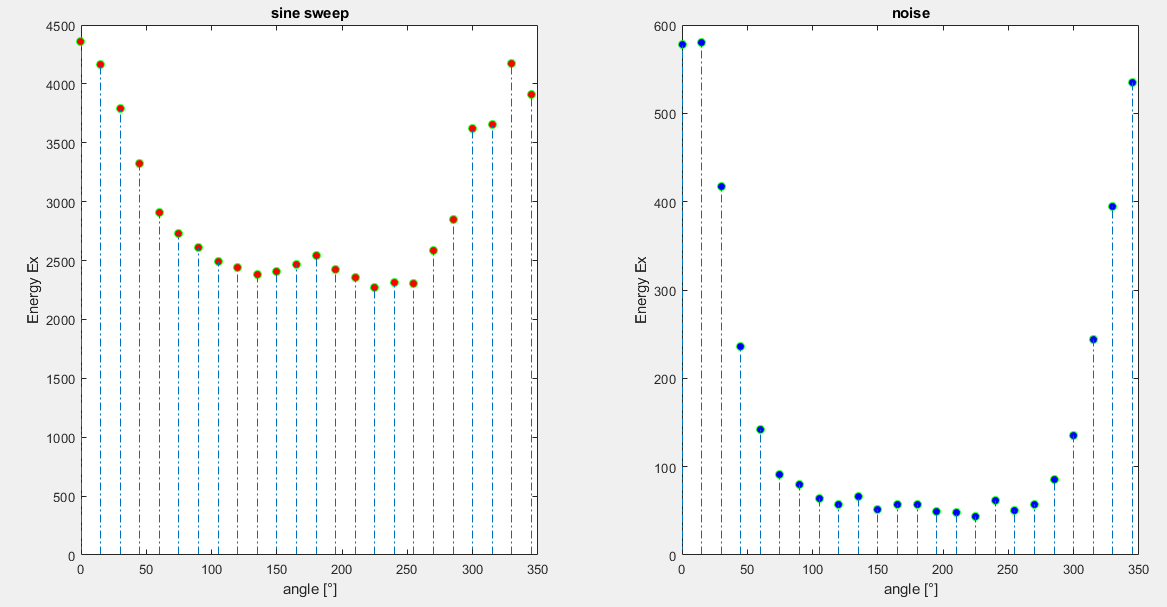
\includegraphics[width=0.75\linewidth]{sig_energy.png}
	\caption{Energies of the recorded signals as functions of the angle of acquisition.}
	\label{fig:energy}
\end{figure}

In \verb|exercise1.m| we label the signals with the angle at which they were recorded and the related type of input. We then compute the energies of the signals with the function\footnote{This function has been added to the provided \texttt{Functions} folder.} shown in List. \ref{list:nrg}. The energies of the sine sweep signals are larger than those of the noise signals, which is expected since the sweep acquisitions were longer (10 vs. 3 seconds). Either way, Fig. \ref{fig:energy} shows that the dependency on the angle is similar, as the energies are larger the closer we are to having the speaker pointed directly towards the microphone. Other specifics of the implementation, in this as in the other exercises, are explained in the comments of the Matlab scripts.

\begin{lstlisting}[language=Matlab, caption=compute\_energy.m, label=list:nrg]
	function [energy] = compute_energy(input)
		len = length(input);
		energy = 0;
		
		for i = 1:len
		energy = energy + abs(input(i))^2;
		end
	
	end
\end{lstlisting}

\section{Room reflection analysis using autocorrelation}
\begin{figure}[h]
	\centering
	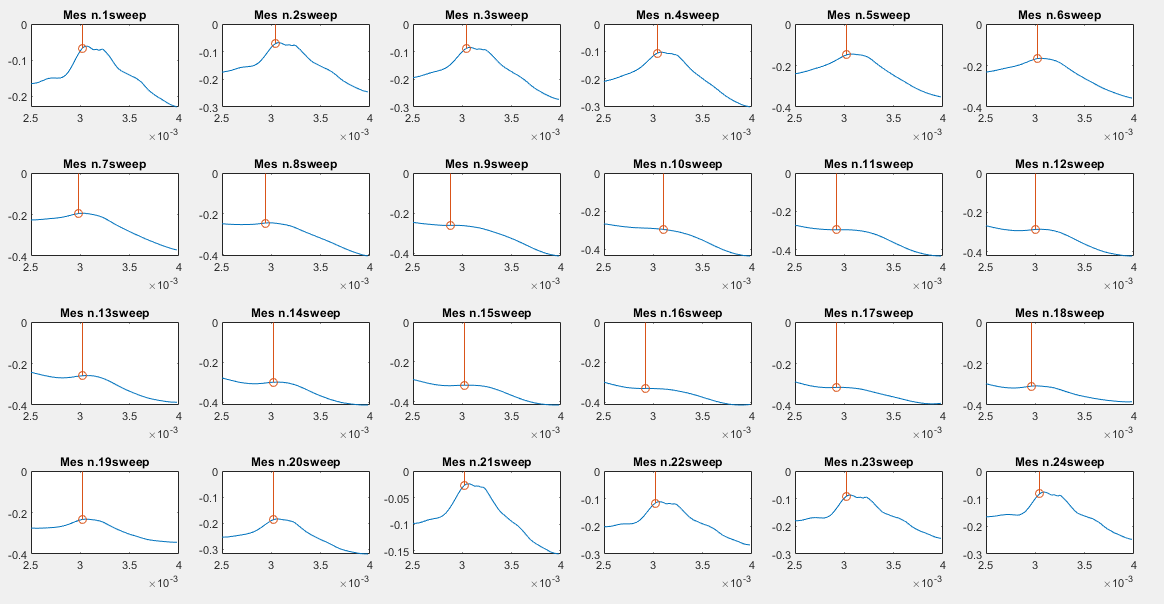
\includegraphics[width=0.85\linewidth]{sweep_peaks.png}
	\caption{First peaks of the autocorrelation functions for the \textbf{sweep signals}. A small portion of the autocorrelation is shown and the stem highlights the position of the peak.}
	\label{fig:sweepcorr}
\end{figure}

\begin{figure}[h]
	\centering
	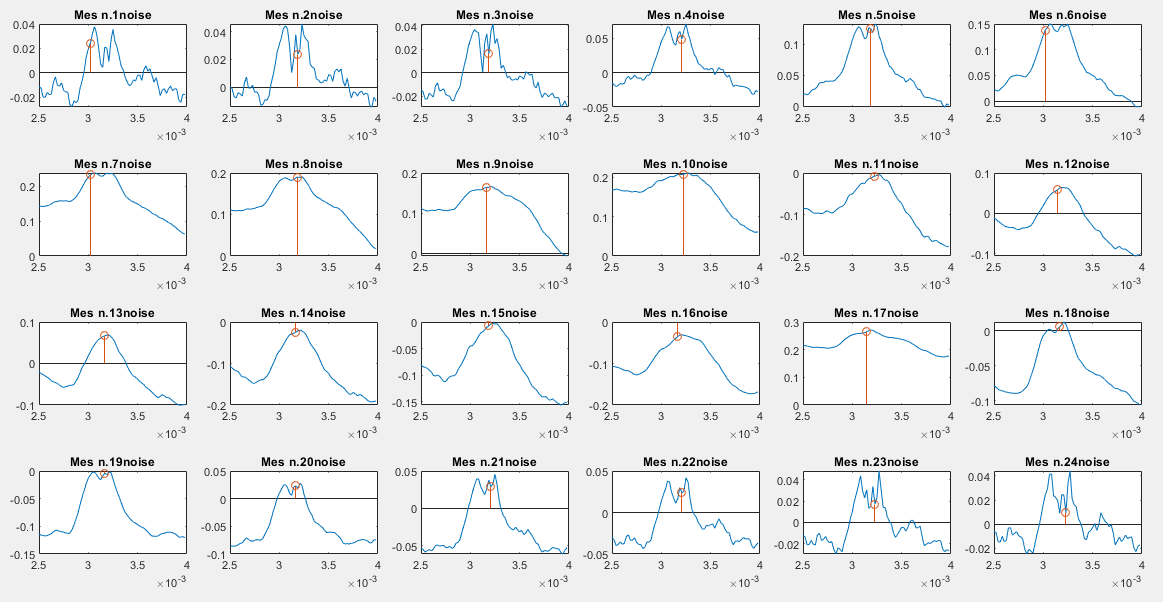
\includegraphics[width=0.85\linewidth]{noise_peaks.png}
	\caption{First peaks of the autocorrelation functions for the \textbf{noise signals}. A small portion of the autocorrelation is shown and the stem highlights the position of the peak.}
	\label{fig:noisecorr}
\end{figure}


In \verb|exercise2.m| we estimate the first reflection time from the autocorrelation of the recorded signals. The autocorrelation is computed and then visualized in order to find the first reflection; a small portion ($\sim$ 2 ms) of the signal around the selected peak is then extracted and the library function \verb|findpeaks| is run on it in order to estimate the exact location of the peak (see Figs. \ref{fig:sweepcorr} and \ref{fig:noisecorr}).

We then find an estimate of the time of arrival of the first reflection by taking the average and standard deviation of the locations of the peaks.  We can use this value to compute the distance of the microphone from the reflector by multiplying them for the speed of sound $c$.The results are reported in Tab. \ref{tab:refl}.
\begin{table}[h!]
	\centering
	$\begin{array}{l|ccc}
		\toprule
		 & \text{\textbf{sweep}} & \text{\textbf{noise}} & \text{\textbf{both}}\\
		 \hline
		 \text{TOA [ms]} & 3.00 \pm 0.05 & 3.20 \pm 0.06 & 3.1 \pm  0.1 \\
		 r\text{ [m]} & 1.03 \pm 0.02 & 1.10 \pm 0.02 & 1.07 \pm 0.03\\
		 \bottomrule
	\end{array}$
	\caption{Estimated time of arrival of the first reflection and microphone-reflector distance. From left to right, the averages over the sweep signals, the noise signals and over the entire set.}
	\label{tab:refl}
\end{table}

\end{document}